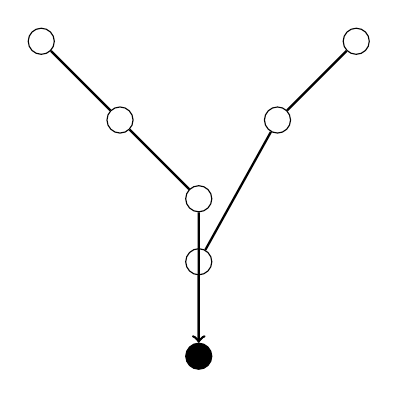
\begin{tikzpicture}[
    sws/.style={circle, fill=white, draw=black, minimum size=5pt},
    snap/.style={circle, fill=black, draw=black, minimum size=7pt},
    arrow/.style={->, thick}
]

\node[sws] (a1) at (-2,1){};
\node[sws] (a2) at (-1,0){};
\node[sws] (a3) at (0,-1){};

\node[sws] (b1) at (2,1){};
\node[sws] (b2) at (1,0){};
\node[sws] (b3) at (0,-1.8){};

\node[snap] (C) at (0,-3) {};

\draw[arrow] (a1)--(a2)--(a3)--(C);
\draw[arrow] (b1)--(b2)--(b3)--(C);

\end{tikzpicture}